%priprava posamezne ure
%tukaj zaporedoma napisemo{st. zaporedne ure}{datum}{naslov}{poglavje}{oblika dela}{pripomocki}
\begin{priprava}{}{}{Zaporedja}{Lastnosti zaporedja}{frontalna}{tabla}

% (končno, neskončno, monotonost, omejenost, konvergentnost …)

Ali imajo naslednja zaporedja kakšne posebne lastnosti? \didopomba{Če ni odziva, kar direkt vprašaš ``ali narašča?'' ipd.}
\begin{align*}
    & -2, -1, 0, 1, 2, 3, 4, 5 \ldots \\
    & 16, 8, 4, 2, 1, \frac{1}{2}, \frac{1}{4}, \frac{1}{8} \ldots \\
    & 1, -1, 2, -2, 3, -3, 4, -4 \ldots \\
    & 2, 0, 1, -1, 0, -2, -1, -3 \ldots
\end{align*}


Glede na urejenost je zaporedje \didopomba{lahko zraven narišeš primere grafov zaporedij, ki ustrezajo tej lastnosti ...}:
\begin{itemize}
    \item \textbf{naraščajoče}, če za $ \forall n \in \NN $ velja $ a_n \leq a_{n+1} $,
    \subitem \textbf{strogo} naraščajoče: $ a_n < a_{n+1} $,
    \begin{figure}[h]
        \centering
        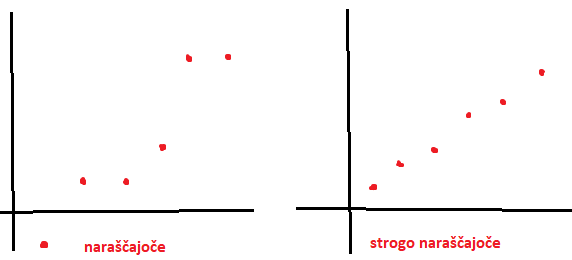
\includegraphics[width=0.5\textwidth]{slike/narascajoce.png}
    \end{figure}
    \item \textbf{padajoče}, če za $ \forall n \in \NN $ velja $ a_n \geq a_{n+1} $,
    \subitem \textbf{strogo} padajoče: $ a_n > a_{n+1} $,
    \begin{figure}[h]
        \centering
        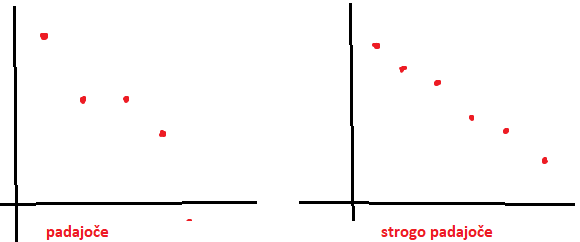
\includegraphics[width=0.5\textwidth]{slike/padajoce.png}
    \end{figure}
    \item \textbf{alternirajoče/spreminjajoče}, če ima vsak naslednji člen nasprotni predznak kot prejšnji,
    \item nič od naštetega (npr. $ 1, 2, 3, 2, 3, 4, 3, 4, 5 \ldots $).
\end{itemize}

\newpage

\begin{figure}[h]
    \centering
    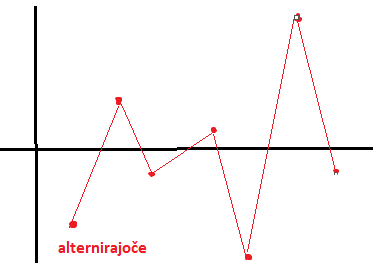
\includegraphics[width=0.3\textwidth]{slike/alternirajoče.png}
    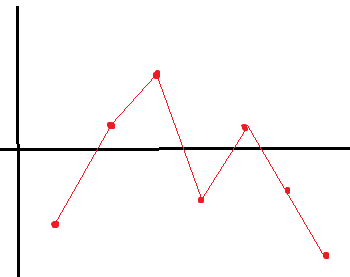
\includegraphics[width=0.3\textwidth]{slike/grdo_zaporedje.png}
\end{figure}

Glede na omejenost je zaporedje \didopomba{začneš s skico in šele potem z $ m $-ji in $ M $-ji}:
\begin{itemize}
    \item \textbf{navzdol omejeno}, če obstaja $ m \in \RR $, da so vsi členi zaporedja večji ali enaki od njega: $ a_n \geq m $ za vsak $ n \in \NN $.
    \item \textbf{navzgor omejeno}, če obstaja $ M \in \RR $, da so vsi členi zaporedja manjši ali enaki od njega: $ a_n \leq M $ za vsak $ n \in \NN $.
    \item \textbf{omejeno}, če je navzdol in navzgor omejeno (obstajata $ m, M \in \RR $, da za vse člene zaporedja velja: $ m \leq a_n \leq M $ za vsak $ n \in \NN $).
    \begin{figure}[h]
        \centering
        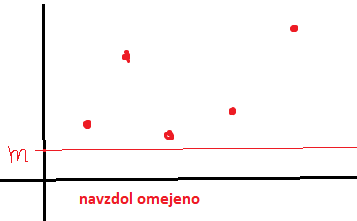
\includegraphics[width=0.3\textwidth]{slike/navzdol.png}
        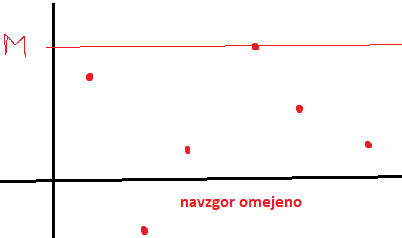
\includegraphics[width=0.3\textwidth]{slike/navzgor.png}
        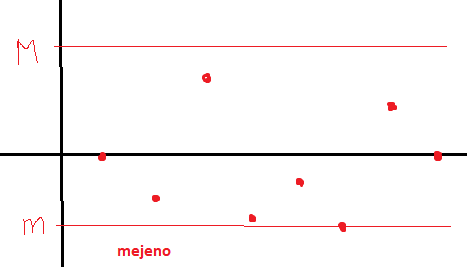
\includegraphics[width=0.3\textwidth]{slike/omejeno.png}
    \end{figure}
\end{itemize}

\vaje{
Vaje:
\begin{itemize}
    \item Dokaz naraščanja/padanja zaporedij (izberi primer, kjer to ni očitno, npr. kakšen racionalen splošni člen \ldots) \didopomba{Torej ali je $ a_n - a_{n-1} \leq $ ali $ \geq 0$}
    \item Preproste ugotovitve npr. Padajoče zaporedje je navzgor omejeno s prvim členom, konstantno zaporedje \didopomba{posebej ga omeni in označi} ni STROGO naraščajoče/padajoče zaporedje
\end{itemize}
}

\end{priprava}